\chapter{Konzept}
\label{cha:konzept}

\section{Kollisionsvermeidung durch kritische Bereiche}
Bei der Analyse des verwendeten Verfahrens zur Bahnplanung entstehen mehrere Bereiche bei den die Potentialfeldmethode an ihre Grenzen stößt. Es treten lokale Minimas auf die nicht gleich mit dem Zielpunkt sind, zwei Roboter können sich bei gleichem Ziel jeweils gegenseitig am erreichen hindern. Hinter den Stationen und links von der ersten Station ist nicht genügend Platz zur perfekten Bahnplanung mittels Potentialen. Würde ein anderer Robotino in die gleich Region fahren, ist die geplante Strecke nur noch schwer zu realisieren. Die Wahrscheinlichkeit, dass der Robotino gegen die Wand oder Station "gedrückt" wird steigt stark. \\
\\
Aus diesem Grund wurden hinter den Stationen Einbahnstraßen entworfen in den der Robotino geschützt wieder in den freien Bereich geführt wird. Hiermit wird jedoch noch nicht das Problem der Roboterbegegnung vor den Zielen verhindert.
\subsection{Selbstorganisation durch Wartebereiche}
\label{subsec:Selbstorga}
Um die Entstehung von lokalen Minima zu verhindern wurde die Software der Robotinos um eine Selbstorganisation erweitert. 
Diese Erweiterung beinhaltet Wartepositionen damit ein Roboter der zur einer bereits besetzten Station fahren soll sich außerhalb des Kollisionsbereichs anstellt.
\begin{figure}[h]
	\centering
	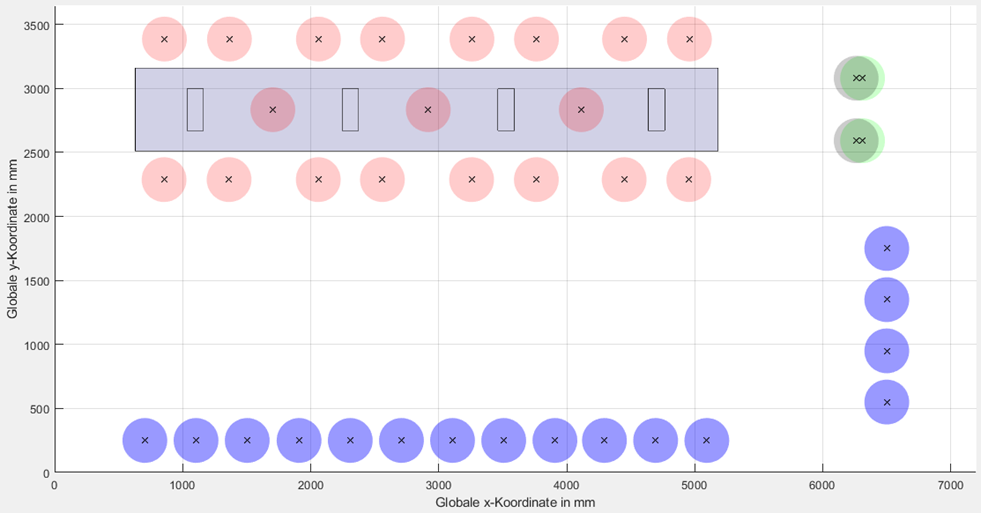
\includegraphics[width=0.5\textwidth]{Bilder/Lageplan.png}
	\caption{Lageplan der FIFO Plätze}
	\label{FIFOPlan}
\end{figure}
\\
In Abbildung \ref{FIFOPlan} erkennt man am unteren Rand der Karte 12 blaue Kreise, welche die Wartebereiche darstellen. Zu jeder Station gehören 3 Wartepositionen. Durch sich verändernde Zählweisen ist der zugehörige Warteplatz zu einer Station immer eindeutig zuzuweisen. Im Kapitel \ref{cha:Implementierung} wird dies weiter erläutert.\\
\\
\\
Mit Hilfe des UDP-Datenpaketes der Kameradaten  ist es für einen Robotino möglich die Positionen der anderen Robotinos zu erhalten. Ist nun die Zielstation bereits von einem anderen Robotino belegt wird mit Hilfe der Selbstorganisationssoftware die erste mögliche Wartepostion als Ziel übernommen. Ist diese auch bereits belegt wird die Warteposition um einen Platz erhöht.\\
Dem gesamten Anstellporzess liegt das First In First Out-Prinzip zu Grunde.( Im weiteren nur noch FIFO genannt.)
Dies bedeutet: Wer sich als erstes anstellt darf auch als erstes wieder herausfahren.\\
Damit auch die Warteschlange beim herausfahren eingehalten wird, wurde die Software ein weiteres mal erweitert.
Die Position der anderen Roboter wird in einem Merker gespeichert und erst zurückgesetzt wenn der Roboter an der nächsten Warteposition bzw. an der Zielposition angekommen ist. Besonders das freischalten der ersten Wartepostion ist kritisch. Wenn ein anderer Robotino die Zielstation verlassen hat, für diese Station aber mehr als ein Robotino wartet, würde beide Robotinos direkt zur Station fahren. Mit Hilfe des Merkers wird die erste Warteposition erst freigeschaltet wenn der Robotino der vorher in der ersten Wartepostion war an der Zielstation angekommen ist. Das bedeutet, dass auch während der längeren Strecke zwischen Wartepositionen und Stationen gesichert ist, dass nur ein Robotino gleichzeitig die Station anfährt. Ist der Roboter dort angekommen wird die erste Wartepostion freigeschaltet und der Robotino auf dem zweiten Platz darf auf den ersten Platz vorfahren.\\
\\
Diese Warteschlange wird noch ein weiteres mal im Progrmmablauf abgefragt. Hat der Robotino seinen Auftrag abgearbeitet, also sein Werkstück abgeholt bzw. abgelegt, wird die Belegung der Warteschlange zur zugehörigen Station abgefragt. Wartet dort bereits der nächste Roboter fährt der Robotino nach Hinten aus der Station heraus. Von dort gelangt er über die Einbahnstraßen wieder in das freie Feld.\\
\\
Bei der Erweiterung des Projektes um einen fünften Roboter wie in Kapitel \ref{cha:Robo2.0} erklärt, wird die vierte Anstellposition nicht neben den anderen Wartepostionen generiert sondern auf Grund von Platzmangel wird als Ziel die Standbyposition einprogrammiert.
 
\subsection{Bekannte Hindernisse}
\label{subsec:bekannt}
Um generelle Begegnungen anderen Robotinos in der normalen Fahrzone zu vermeiden wurde ein Ausweichmanöver entworfen. 
Befindet sich ein anderer Roboter im Bereich zwischen den gesteuerten Roboter und seinem Ziel und in einer Entfernung von 20 cm wird auf den Zielvektor eine $90^\circ$-Drehung addiert. Der Robotino fährt somit für eine kurze Zeit mit gleichbleibenden Abstand zum Ziel. Ist der behindernde Robotino nicht mehr im gefährdeten Bereich wird wieder der normale Zielvektor eingestellt.\\
\\
Für eine hohe Dynamik im Gesamtsystem unterscheidet die Software zwischen sich bewegenden Robtinos und stehenden. Anhand der Kameradaten werden die aktuellen Positionen mit deren vorherigen mittels Merker verglichen. Ist die Differenz größer der Toleranz bewegt sich der Robotino. Sich bewegende Robotinos stelle eine größere Kollisionsgefahr dar. Deshalb werden die Potentialfelder jener Robotinos vergrößert. Der gesteuerte Roboter wird somit in einem größeren Abstand vorbei fahren.

\subsection{Unbekannte Hindernisse}

Das verbaute Kamerasystem ist nicht in der Lage andere Objekte, außer die mit Aruko-Markern versehenden Robotinos, zu erkennen. Um jedoch auch eine Kollision mit Menschen zuverhindern besitzt der Robotino 9 Infrarot-Sensoren gleichmäßig um den untersten Rand des Roboters verteilt. Detektiert einer der Sensoren ein Objekt ermittelt die Software an welcher Stelle das Objekt erkannt wurde und manipuliert den Zielvektor. Es wird ein um $180^\circ$ gedrehter Zielvektor ein programmiert.
Hat sich das unbekannte Hindernis entfernt wird wieder der normale Zielvektor geschaltet.
\newpage
\section{Schnittstellen}
Im gesamten Projektablauf ist die Kommunikation mit anderen Gruppen ausschlaggebend für eine perfektes Gesamtkonzept.
In der Bahnplanung wurde vorallem mit der Gruppe der Bahnregelung und mit der Gruppe der Fertigungsplanung eng zusammengearbeitet.
\subsection{Bahnregelung}
In sehr engen Bereichen in denen auch noch eine hohe Präzision erforderlich ist stößt die Potentialfeldmethode an ihre Grenzen. Aus diesem Grund wurde der gesamte Bereich direkt am Anfang des Projektes aufgeteilt. Das Potentialfeld wird in den freien Bereiche benutzt und an den Randbereichen des Feldes. Das Anfahren der einzelnen Fächer innerhalb der Stationen sowie das Werkstückhandling ist an die Bahnregelung übergeben worden.\\
\\
In Abbildung \ref{FIFOPlan} stellen die 8 roten Kreise vor den Stationen die Übergabepunkte da. Befindet sich der Robotino innerhalb eines solchen Kreises, inklusive einer gewissen Toleranz, wird ein Übergabe Bit gesetzt und die Bahnregelung übernimmt das präzise Anfahren zuerst des RFID Lesegerätes und anschließend das Ablegen in ein Stationsfach. ( Beim Abholen ist der Prozess andersherum.)
Somit gehören zur Schnittstelle nicht nur der Übergabebit. Die Gruppe der Bahnregelung benötigt darüber hinaus auch noch den genauen Auftrag der Fertigungsplanung. Hat die Bahnregelung den Auftrag abgearbeitet wird der Übergabebit am Übergabepunkt getoggelt und der Robotino fährt wieder im Potentialfeld. Dieser Übergabepunkt ist variabel wie bereits in dem Unterkapitel \ref{subsec:Selbstorga} erläutert.\\
\\  
Da die Bahnregelung sehr präzise die Position des Robotinos für eine hoch genaue Fahrt benötigt, wurde von der Gruppe ein Kalman-Filter für die Robotino Position entworfen. Ohne Beobachter sendet die Kamera bei nicht Erkennung eines Robotinos die Positionsdaten [0,0]. Diese falsche Postion kann zu einigen Fehlern in den Berechnungen führen. Dieser Beobachter ermöglicht eine Fehlerfreie Positionsdarstellung des Roboters auch bei kurzzeitiger Verdeckung des Arukomarkers. Die Beobachterdaten werden auch in der Bahnplanung durchgehende verwendet. 
\newpage
\subsection{Fertigungsplanung}
Die Fertigungsplanung ist für die gesamte Simulation der Fabrikumgebung zuständig. In der Gruppe werden verschiedene Aufträge generiert und intelligent auf die vier Robotinos verteilt. Mittels UDP Kommunikation wird der jeweilige Auftrag an den jeweiligen Roboter gesendet.
\begin{figure}[h]
	\centering
	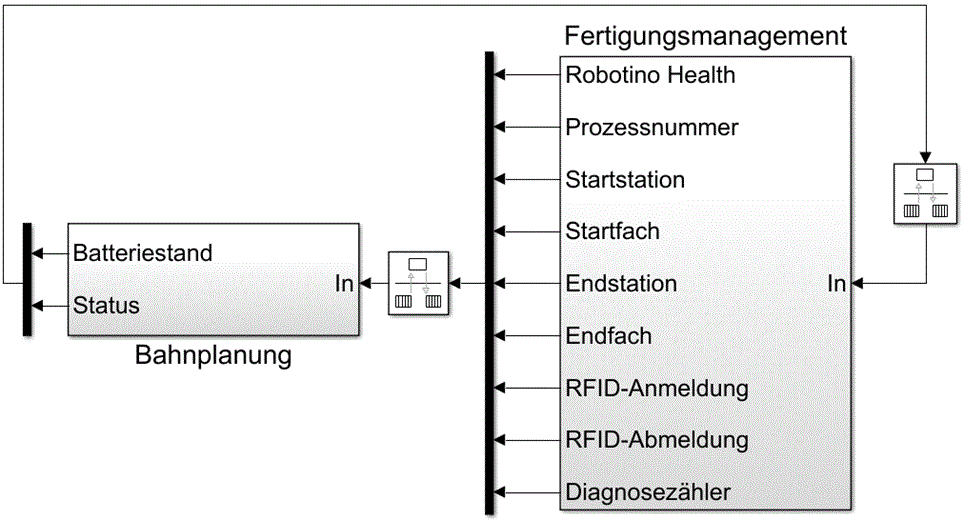
\includegraphics[width=0.6\textwidth]{Bilder/Schnittstelle_Fertigungsplanung.png}
	\caption{Schnittstelle mit der Fertigungsplanung}
	\label{pic:SchnittstelleGewerk1}
\end{figure}
\noindent
In Abbildung \ref{pic:SchnittstelleGewerk1} ist der Informationsaustausch dargestellt. Die Informationen, die die  Bahnplanung an die Fertigunsplanung zurücksendet, wurden um einen weiteren Punkt erweitert. Die Ist-Position des Roboters wird ebenfalls gesendet. Diese Position wird von der Fertigungsplanung für die Fabriksimulation benötigt. Im Status Byte wird übermittel was der Robotino zu dem Zeitpunkt gerade ausführt. Also ob er im Potentialfeld fährt oder eine Stationanfährt, etwas ablegt bzw. etwas aufnimmt. Darüber hinaus werden im Status auf Fehlermeldungen weitergeleitet, dazu im Unterkapitel \ref{Fehlererkennung} mehr.\\
\\
Von der Fertigungsplanung bekommt das Programm den genauen Auftrag den der Robotino abarbeiten soll. Jeder neue Auftrag erhält auch eine neue Prozessnummer. Der Auftrag besteht aus der Startstation mit zugehörigem Fach, an dem ein Werkstück abgeholt werden soll, und in welches Fach von welcher Station es gebracht werden soll. 
Damit jedes individuelle Werkstück auch entsprechend erkannt wird, sind an jeder Station RFID Lese-/Schreibköpfe angebracht. Wird ein Werkstück in die jeweilige Station gebracht wird es dort angemeldet. Beim  Aufnehmen wird es abgemeldet. Hierfür werden zwei Bytes in der Schnittstelle verwendet. Die Information über die einzelnen Werkstücke werden von der Fertigungsplanung verarbeitet und in einer Cloud gespeichert.\\
\newpage

\subsection{Fehlererkennung}
\label{Fehlererkennung}

Eine weitere Übergabeinformation zwischen den drei Gruppen ist das Fehlerhandling. Es wird zwischen drei verschiedenen Fehlern des Robotinos unterschieden:
\begin{enumerate}
\label{Fehlerliste}
\item Kein Werkstück vorhanden
\item Stationsfach belegt
\item Werkstück verloren
\end{enumerate}
\noindent
Beim Anfahren eines Stationsfachs zur Aufnahme eines Werkstückes durch die Bahnregelung wird zwischen den Greifern eine Lichtschranke abgefragt. Ist diese Lichtschranke beim schließen des Greifers nicht durchbrochen wird der erste Fehler ausgelöst. Dieser Fehler wird anschließend an die Fertigunsplanung gesendet. Die Fertigungsplanung entscheidet dann ob ein falscher Auftrag gesendet wurde oder in der 'Fabrik' ein Fehler vorliegt, welcher per manuellen Eingriff behoben werden muss. 
Der zweite Fehler wird über einen Zähler der Anfahrversuche fpr ein Fach realisiert. Schafft der Robotino innerhalb von drei Anfahrversuchen es nicht das Werkstück abzulegen so wird der zweite Fehler gesendet. 
Verliert der Roboter während der Fahrt, auch im Potentialfeld, das Werkstück wird der dritte Fehler gesendet. Hier muss manuell das Werkstück aus dem Fahrbereich entfernt werden.